\documentclass{article}
\usepackage{amsmath}
\usepackage{graphicx}  % Paquete para incluir imágenes
\usepackage{float}
\usepackage{amsmath,amssymb}
\begin{document}
Alberto Arath Figueroa Salomon

Tarea
\section{Ecuación del Plano y una Recta}
\begin{center}
Forma parametrica ecuación de una recta
\[
\mathbf{r} = \mathbf{r}_0 + \lambda\,\mathbf{d},\quad
\]
Forma slope y punto
\[
y = m x + b
\]
Ecuacion vectorial de un plano
% Point-normal form of a plane
\[
    (\mathbf{r} - \mathbf{r}_0) \cdot \mathbf{n} = 0
    \]
    
\end{center}


\section{Descripción de superficies}
\textbf{a) } $1 + x_1 + x_2$  
\begin{itemize}
    \item Cruce con ejes $(-1, 0, 0)$, $(0, -1, 0)$, $(0, 0, 1)$, por lo que no cruza con el origen.
    \item Recta de intersección con el plano $x_1x_2$: $1 + x_1 + x_2 = 0$.
    \item La pendiente de la recta de intersección con el plano $x_1x_2$: $-1$.
    \item Región $x_1x_2$ donde $w^T x > 0$.
    \item Todos los puntos que satisfacen $1 + x_1 + x_2 > 0$ representan la región positiva del plano $w^T x$.
    \item Todos los puntos que satisfacen $1 + x_1 + x_2 < 0$ representan la región negativa del plano $w^T x$.
\end{itemize}
\begin{figure}[H]
    \centering
    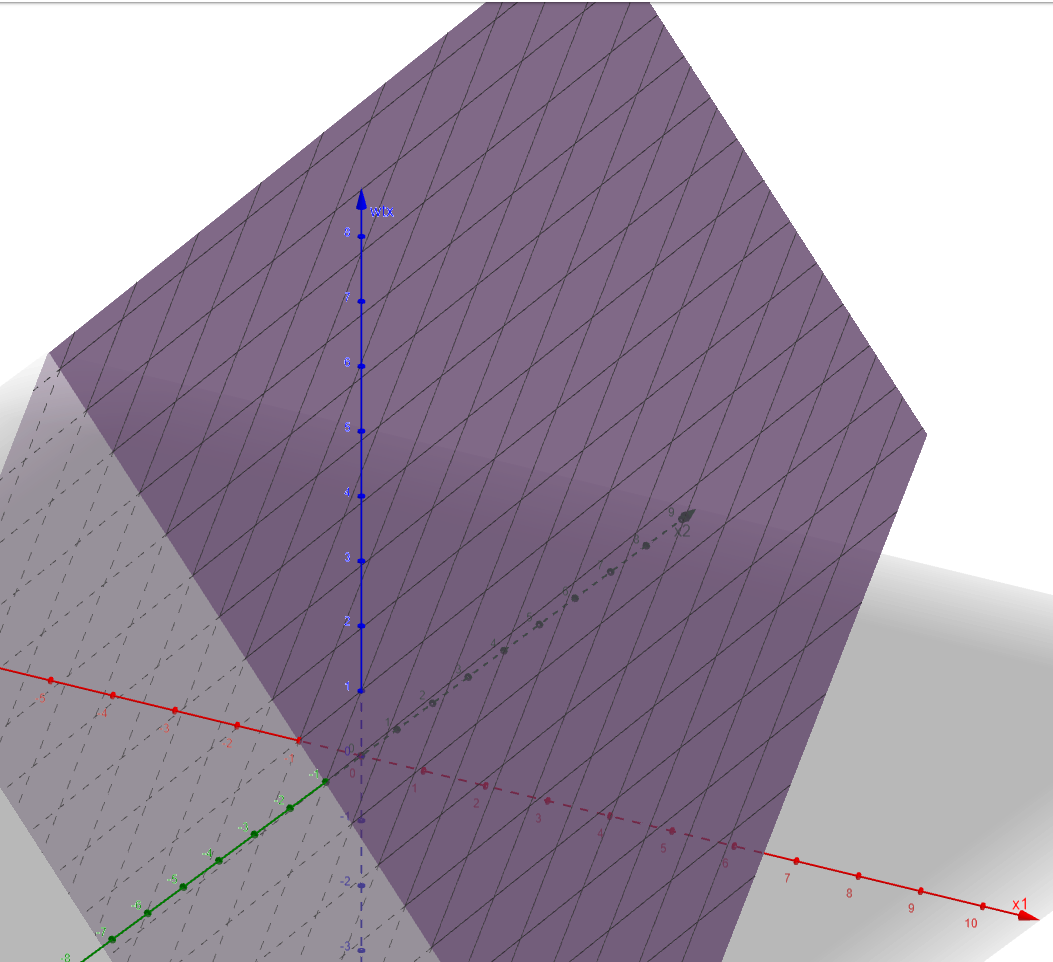
\includegraphics[width=0.5\textwidth]{Imagen1.png}  % Cambia el nombre del archivo y su ruta según sea necesario
\end{figure}

\textbf{b) } $-2 + x_1 + x_2$  
\begin{itemize}
    \item Cruce con ejes $(2, 0, 0)$, $(0, 2, 0)$, $(0, 0, -2)$, por lo que no cruza con el origen.
    \item Recta de intersección con el plano $x_1x_2$: $-2 + x_1 + x_2 = 0$.
    \item La pendiente de la recta de intersección con el plano $x_1x_2$: $-1$.
    \item Región $x_1x_2$ donde $w^T x > 0$.
    \item Todos los puntos que satisfacen $-2 + x_1 + x_2 > 0$ representan la región positiva del plano $w^T x$.
    \item Todos los puntos que satisfacen $-2 + x_1 + x_2 < 0$ representan la región negativa del plano $w^T x$.
\end{itemize}
\begin{figure}[H]
    \centering
    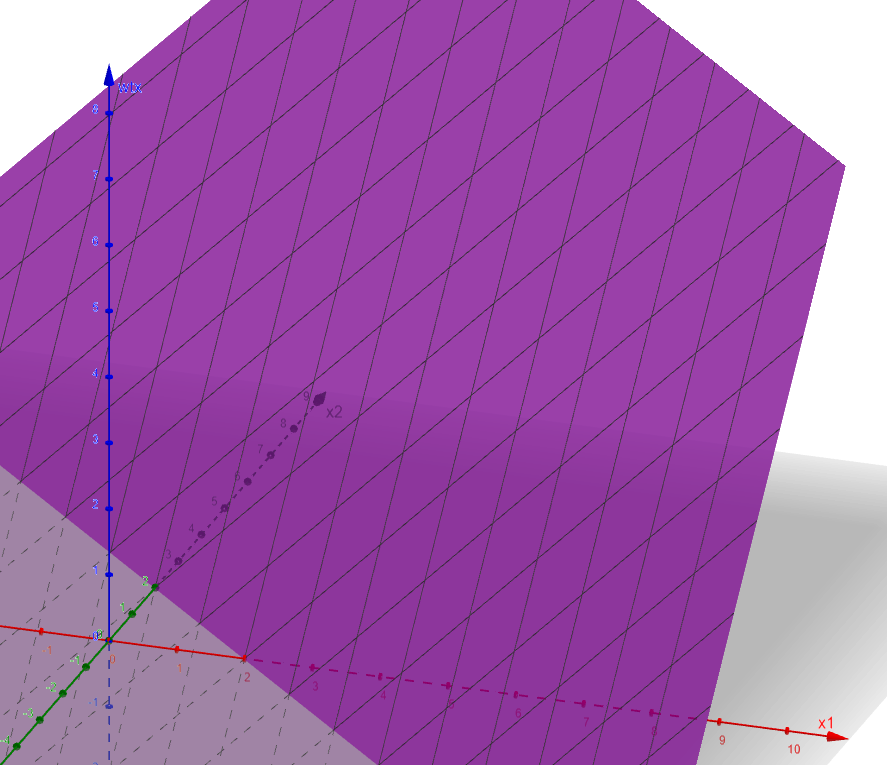
\includegraphics[width=0.5\textwidth]{Imagen2.png}  % Cambia el nombre del archivo y su ruta según sea necesario
\end{figure}
\textbf{c) } $x_1 + x_2$  
\begin{itemize}
    \item Cruza con el origen $(0, 0, 0)$.
    \item Recta de intersección con el plano $x_1x_2$: $x_1 + x_2 = 0$.
    \item La pendiente de la recta de intersección con el plano $x_1x_2$: $-1$.
    \item Región $x_1x_2$ donde $w^T x > 0$.
    \item Todos los puntos que satisfacen $x_1 + x_2 > 0$ representan la región positiva del plano $w^T x$.
    \item Todos los puntos que satisfacen $x_1 + x_2 < 0$ representan la región negativa del plano $w^T x$.
\end{itemize}
\begin{figure}[H]
    \centering
    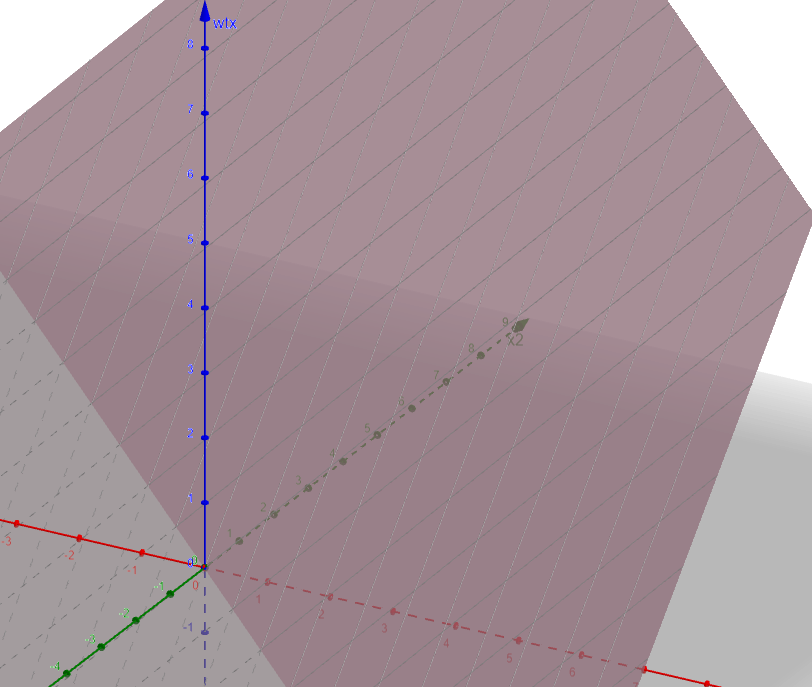
\includegraphics[width=0.5\textwidth]{Imagen3.png}  % Cambia el nombre del archivo y su ruta según sea necesario
\end{figure}
\textbf{d) } $1 + 2x_1 + x_2$  
\begin{itemize}
    \item Cruce con ejes $(-1/2, 0, 0)$, $(0, -1, 0)$, $(0, 0, 1)$, por lo que no cruza con el origen.
    \item Recta de intersección con el plano $x_1x_2$: $1 + 2x_1 + x_2 = 0$.
    \item La pendiente de la recta de intersección con el plano $x_1x_2$: $-1/2$.
    \item Región $x_1x_2$ donde $w^T x > 0$.
    \item Todos los puntos que satisfacen $1 + 2x_1 + x_2 > 0$ representan la región positiva del plano $w^T x$.
    \item Todos los puntos que satisfacen $1 + 2x_1 + x_2 < 0$ representan la región negativa del plano $w^T x$.
\end{itemize}
\begin{figure}[H]
    \centering
    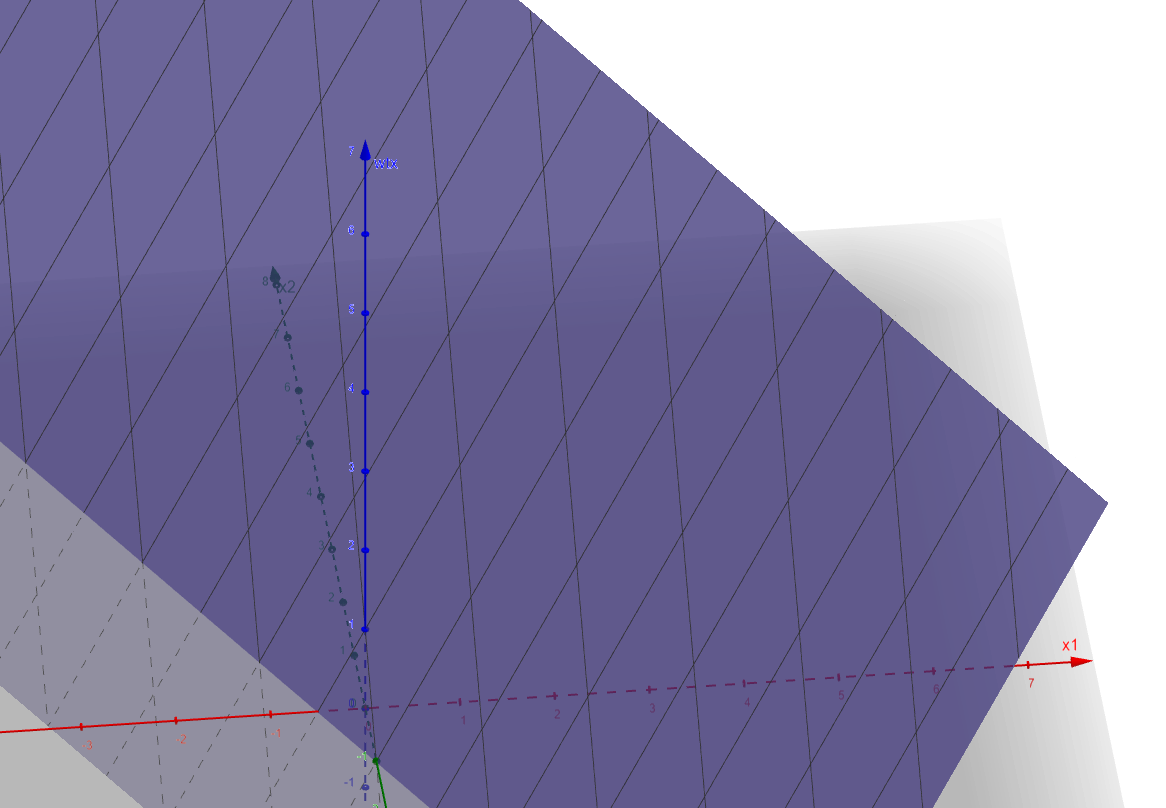
\includegraphics[width=0.5\textwidth]{Imagen4.png}  % Cambia el nombre del archivo y su ruta según sea necesario
\end{figure}
\textbf{e) } $1 - 2x_1 + x_2$  
\begin{itemize}
    \item Cruce con ejes $(1/2, 0, 0)$, $(0, -1, 0)$, $(0, 0, 1)$, por lo que no cruza con el origen.
    \item Recta de intersección con el plano $x_1x_2$: $1 - 2x_1 + x_2 = 0$.
    \item La pendiente de la recta de intersección con el plano $x_1x_2$: $2$.
    \item Región $x_1x_2$ donde $w^T x > 0$.
    \item Todos los puntos que satisfacen $1 - 2x_1 + x_2 > 0$ representan la región positiva del plano $w^T x$.
    \item Todos los puntos que satisfacen $1 - 2x_1 + x_2 < 0$ representan la región negativa del plano $w^T x$.
\end{itemize}
\begin{figure}[H]
    \centering
    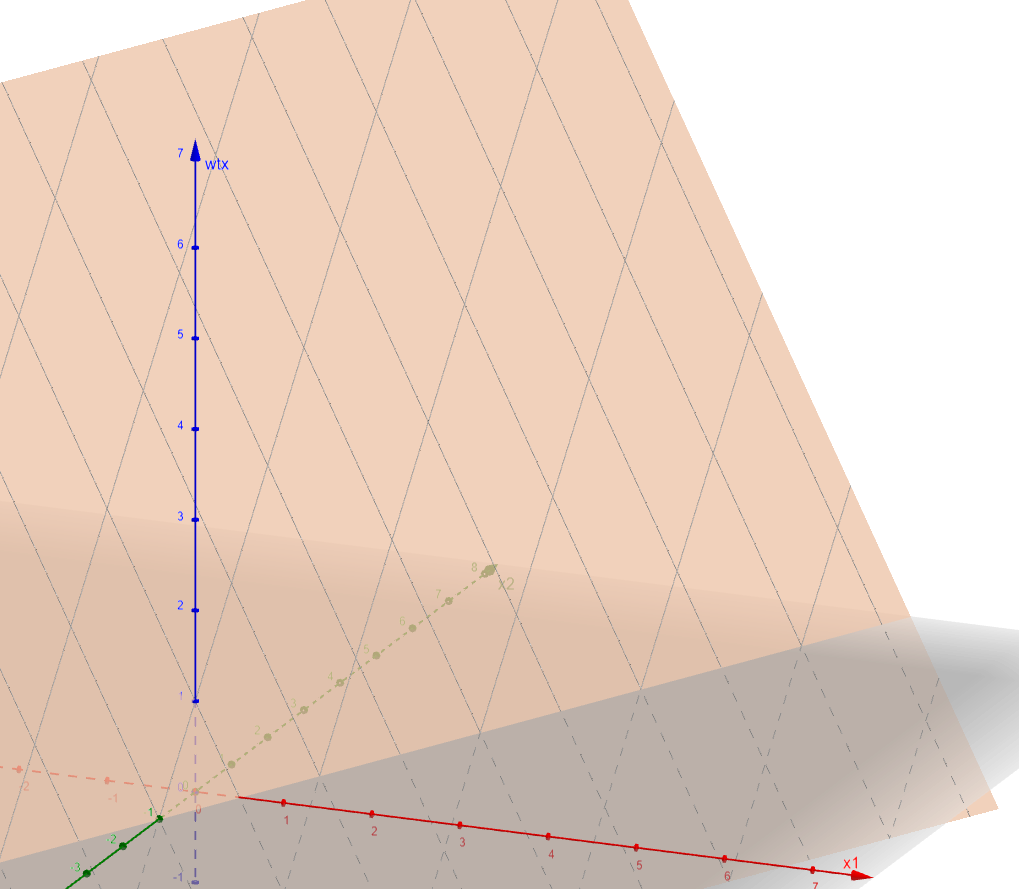
\includegraphics[width=0.5\textwidth]{Imagen5.png}  % Cambia el nombre del archivo y su ruta según sea necesario
\end{figure}
\textbf{f) } $1 + x_2$  
\begin{itemize}
    \item Cruza con ejes $(0, -1, 0)$, $(0, 0, 1)$, por lo que \textbf{no cruza con el eje $x_1$}.
    \item Recta de intersección con el plano $x_1x_2$: $1 + x_2 = 0$.
    \item La pendiente de la recta de intersección con el plano $x_1x_2$: $0$.
    \item Región $x_1x_2$ donde $w^T x > 0$.
    \item Todos los puntos que satisfacen $1 + x_2 > 0$ representan la región positiva del plano $w^T x$.
    \item Todos los puntos que satisfacen $1 + x_2 < 0$ representan la región negativa del plano $w^T x$.
\end{itemize}
\begin{figure}[H]
    \centering
    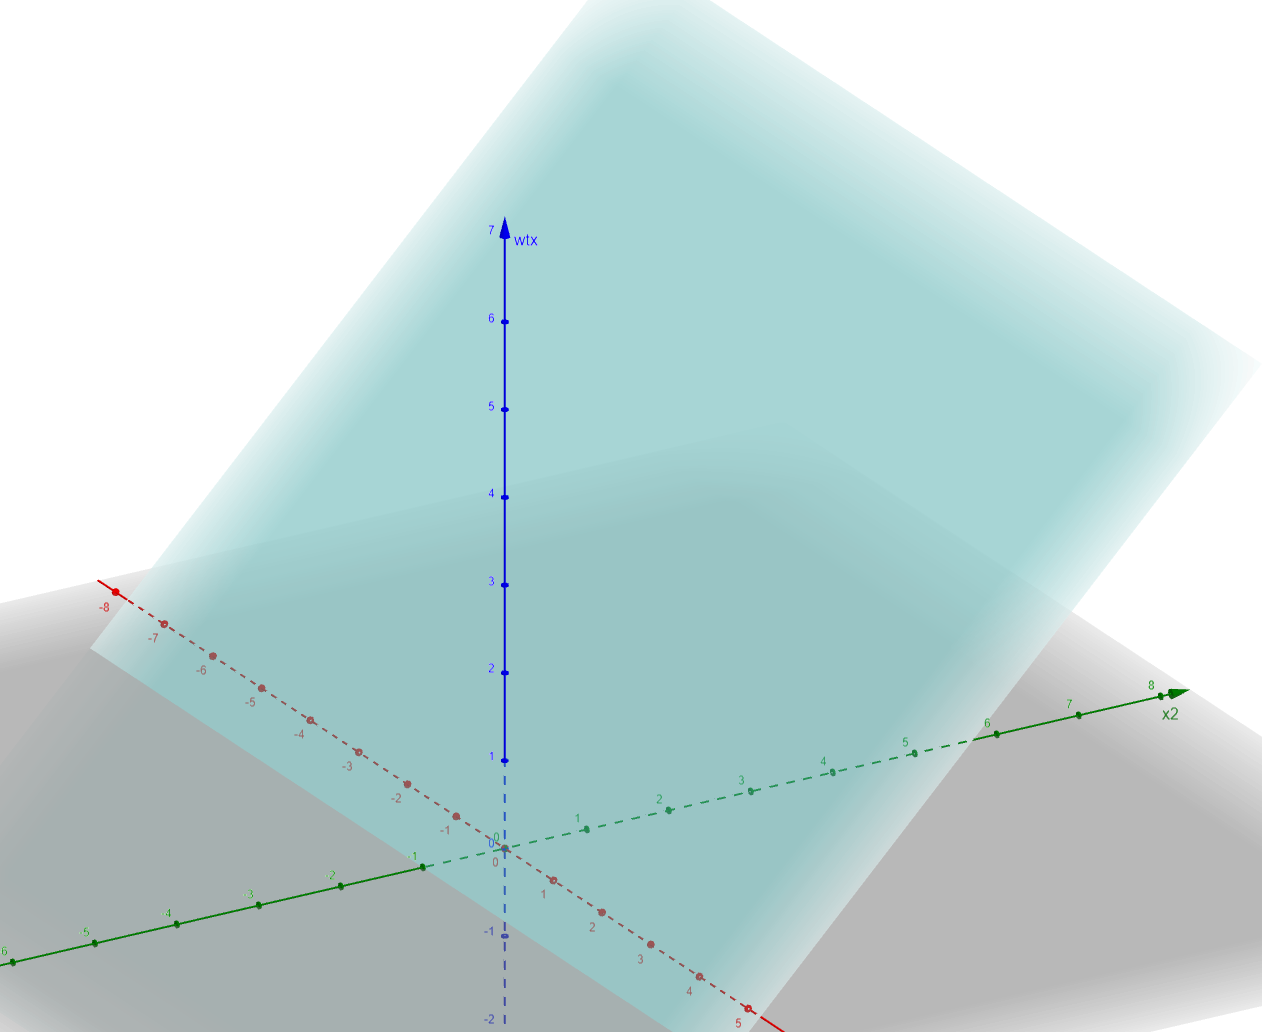
\includegraphics[width=0.5\textwidth]{Imagen6.png}  % Cambia el nombre del archivo y su ruta según sea necesario
\end{figure}
\textbf{g) } $1 + x_1 + 2x_2$  
\begin{itemize}
    \item Cruce con ejes $(-1, 0, 0)$, $(0, -1/2, 0)$, $(0, 0, 1)$, por lo que no cruza con el origen.
    \item Recta de intersección con el plano $x_1x_2$: $1 + x_1 + 2x_2 = 0$.
    \item La pendiente de la recta de intersección con el plano $x_1x_2$: $-1/2$.
    \item Región $x_1x_2$ donde $w^T x > 0$.
    \item Todos los puntos que satisfacen $1 + x_1 + 2x_2 > 0$ representan la región positiva del plano $w^T x$.
    \item Todos los puntos que satisfacen $1 + x_1 + 2x_2 < 0$ representan la región negativa del plano $w^T x$.
\end{itemize}
\begin{figure}[H]
    \centering
    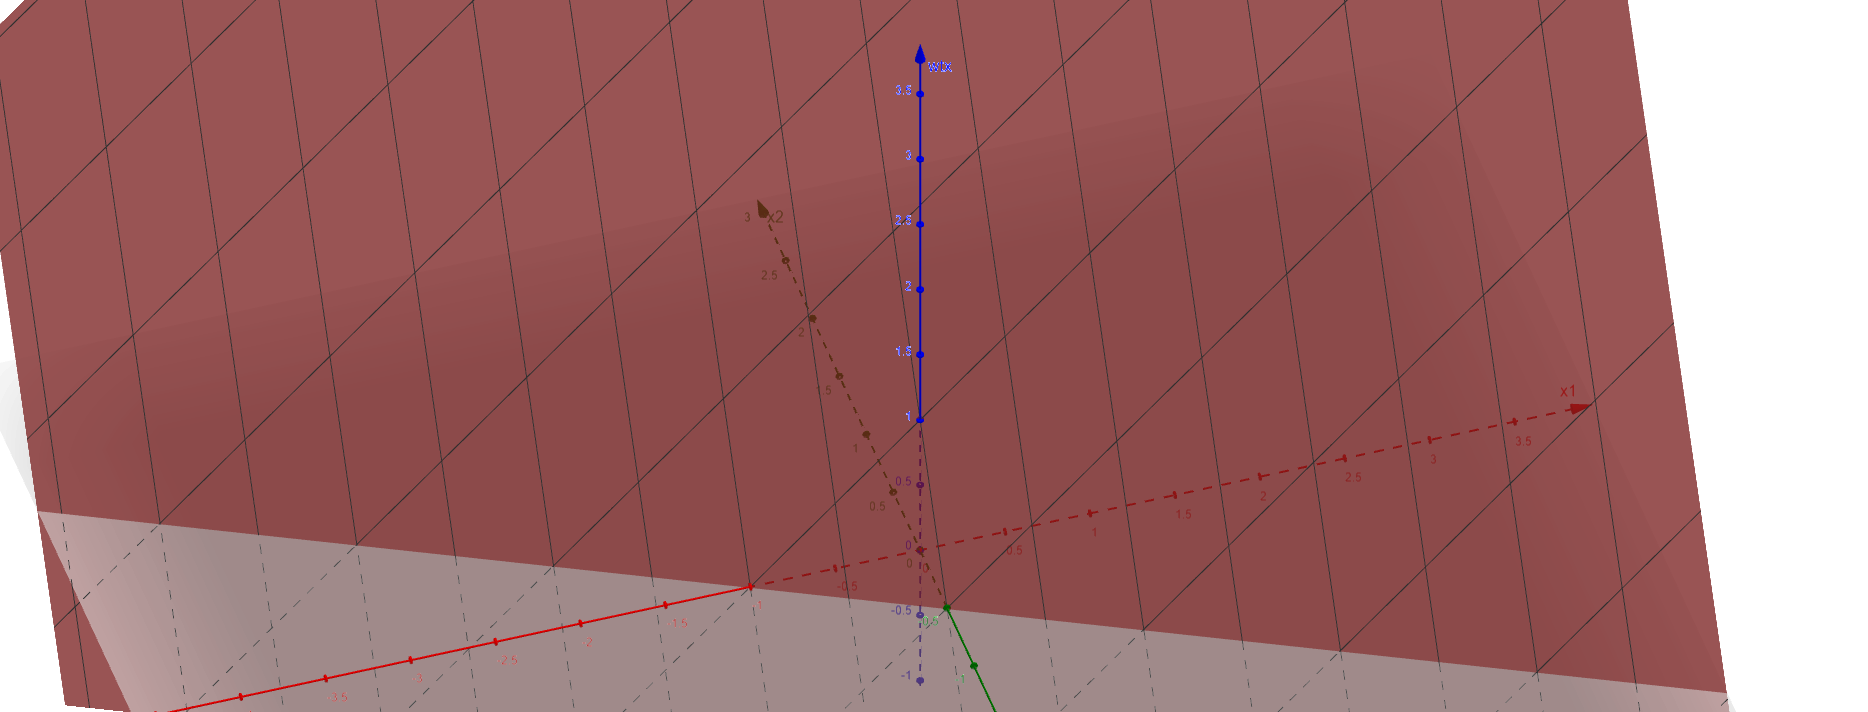
\includegraphics[width=0.5\textwidth]{Imagen7.png}  % Cambia el nombre del archivo y su ruta según sea necesario
\end{figure}
\textbf{h) } $1 + x_1 - 2x_2$  
\begin{itemize}
    \item Cruce con ejes $(-1, 0, 0)$, $(0, 1/2, 0)$, $(0, 0, 1)$, por lo que no cruza con el origen.
    \item Recta de intersección con el plano $x_1x_2$: $1 + x_1 - 2x_2 = 0$.
    \item La pendiente de la recta de intersección con el plano $x_1x_2$: $2$.
    \item Región $x_1x_2$ donde $w^T x > 0$.
    \item Todos los puntos que satisfacen $1 + x_1 - 2x_2 > 0$ representan la región positiva del plano $w^T x$.
    \item Todos los puntos que satisfacen $1 + x_1 - 2x_2 < 0$ representan la región negativa del plano $w^T x$.
\end{itemize}
\begin{figure}[H]
    \centering
    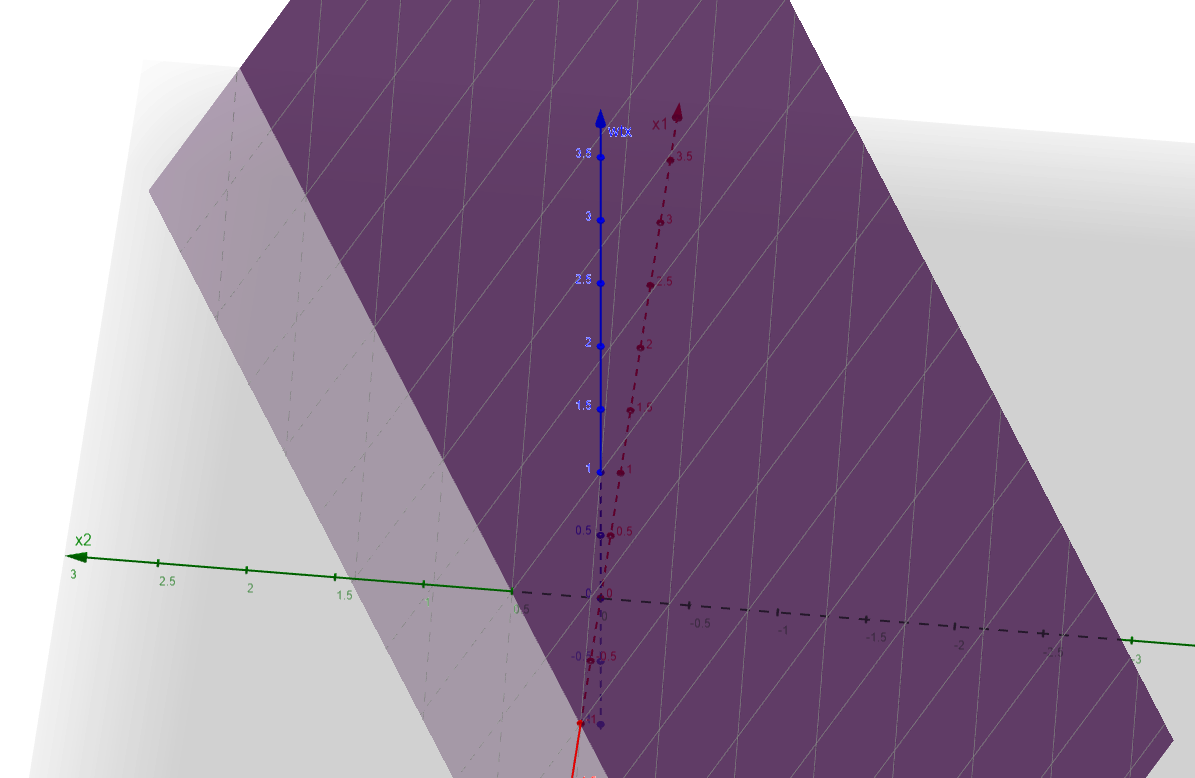
\includegraphics[width=0.5\textwidth]{Imagen8.png}  % Cambia el nombre del archivo y su ruta según sea necesario
\end{figure}
\textbf{i) } $1 + x_1$  
\begin{itemize}
    \item Cruza con ejes $(-1, 0, 0)$ $(0, 0, 1)$, por lo que no cruza con el origen.
    \item Recta de intersección con el plano $x_1x_2$: $1 + x_1 = 0$.
    \item La pendiente de la recta de intersección con el plano $x_1x_2$: $0$.
    \item Región $x_1x_2$ donde $w^T x > 0$.
    \item Todos los puntos que satisfacen $1 + x_1 > 0$ representan la región positiva del plano $w^T x$.
    \item Todos los puntos que satisfacen $1 + x_1 < 0$ representan la región negativa del plano $w^T x$.
\end{itemize}
\begin{figure}[H]
    \centering
    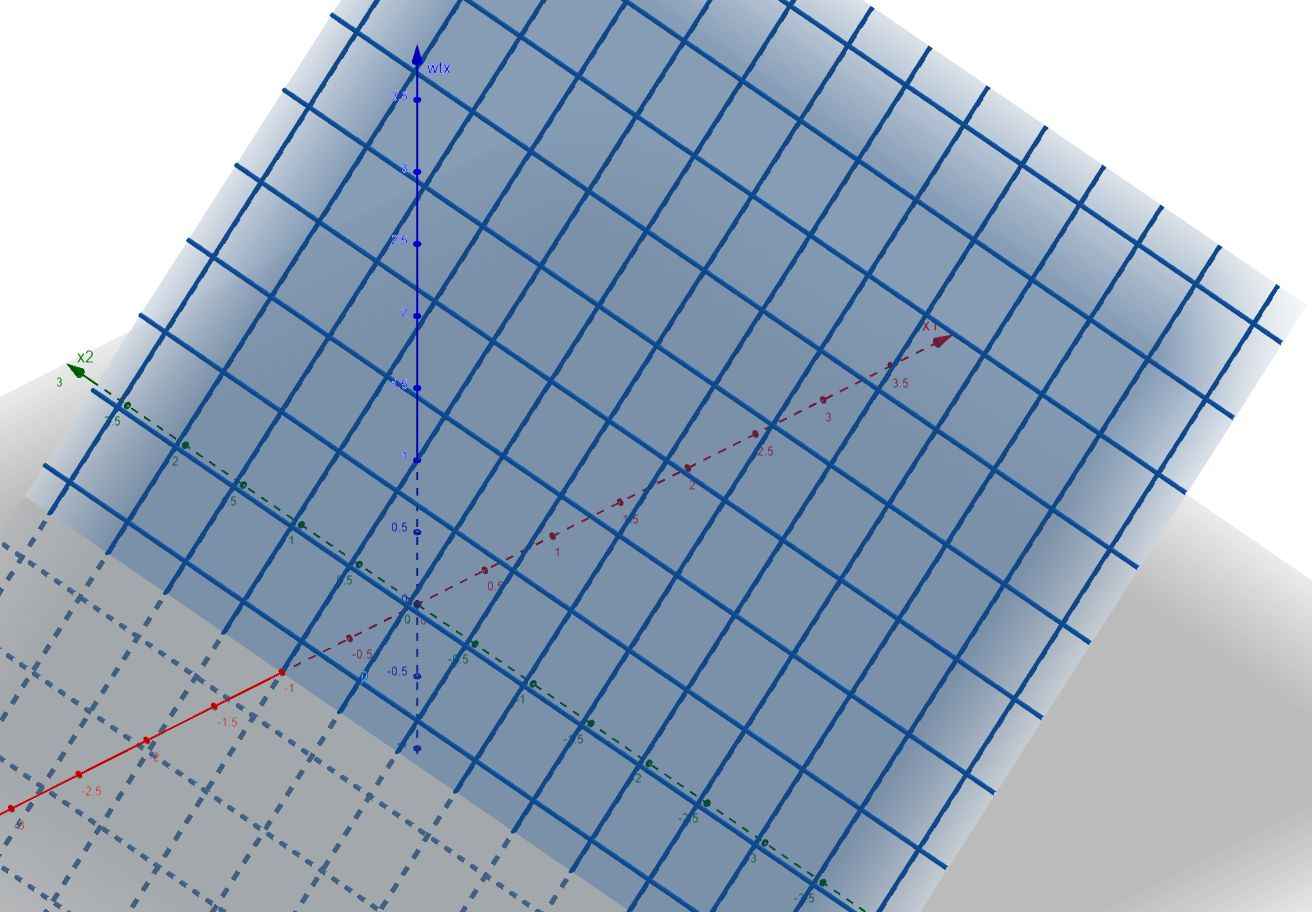
\includegraphics[width=0.5\textwidth]{Imagen9.png}  % Cambia el nombre del archivo y su ruta según sea necesario
\end{figure}


\section{Verificando la ecuación del plano}
Dado que las expresiones representan ecuaciones de planos en la forma:
\begin{equation}
    z = f(x, y)
\end{equation}
para encontrar el vector normal a cada plano, seguimos estos pasos:
\begin{enumerate}
    \item Elegimos tres puntos en el plano.
    \item Formamos dos vectores a partir de estos puntos.
    \item Calculamos el producto cruzado de estos vectores para obtener el vector normal.
\end{enumerate}

\subsection{Para $z = 1 + x + y$}
Puntos elegidos: \\ 
$P_1 = (0,0,1)$, $P_2 = (1,0,2)$, $P_3 = (0,1,2)$ \\[1mm]
Vectores:
\begin{equation*}
    \overrightarrow{P_1P_2} = (1,0,1), \quad \overrightarrow{P_1P_3} = (0,1,1)
\end{equation*}
Cálculo del producto cruzado:
\begin{equation*}
    \mathbf{N} = \overrightarrow{P_1P_2} \times \overrightarrow{P_1P_3} =
    \begin{vmatrix} 
    \mathbf{i} & \mathbf{j} & \mathbf{k} \\
    1 & 0 & 1 \\
    0 & 1 & 1
    \end{vmatrix} = (-1,\,-1,\,1)
\end{equation*}
Ahora, utilizamos la definición de la ecuación del plano:
\[
\mathbf{n} \cdot (\mathbf{r} - \mathbf{p}) = 0
\]
Donde \( \mathbf{n} = (-1,\,-1,\,1) \) y \( \mathbf{p} = (0,0,1) \). Como
\[
\mathbf{r} - \mathbf{p} = (x,\,y,\,z-1),
\]
el producto punto se escribe:
\[
-1\cdot x - 1\cdot y + 1\cdot (z-1)=0.
\]
Simplificando:
\[
-x - y + z - 1 = 0,
\]
o equivalentemente:
\[
x + y - z = -1.
\]

\subsection{Para $z = -2 + x + y$}
Puntos elegidos: \\ 
$P_1 = (0,0,-2)$, $P_2 = (1,0,-1)$, $P_3 = (0,1,-1)$ \\[1mm]
Vectores:
\begin{equation*}
    \overrightarrow{P_1P_2} = (1,0,1), \quad \overrightarrow{P_1P_3} = (0,1,1)
\end{equation*}
Cálculo del producto cruzado:
\begin{equation*}
    \mathbf{N} = \overrightarrow{P_1P_2} \times \overrightarrow{P_1P_3} =
    \begin{vmatrix} 
    \mathbf{i} & \mathbf{j} & \mathbf{k} \\
    1 & 0 & 1 \\
    0 & 1 & 1
    \end{vmatrix} = (-1,\,-1,\,1)
\end{equation*}
Utilizando \( \mathbf{p} = (0,0,-2) \), tenemos:
\[
-1\cdot (x-0) - 1\cdot (y-0) + 1\cdot \bigl(z-(-2)\bigr)=0,
\]
lo que se traduce en:
\[
-x - y + z + 2 = 0,
\]
y al reordenar:
\[
z = x + y - 2 \quad \Longleftrightarrow \quad x+y-z=2.
\]

\subsection{Para $z = x + y$}
Puntos elegidos: \\ 
$P_1 = (0,0,0)$, $P_2 = (1,0,1)$, $P_3 = (0,1,1)$ \\[1mm]
Vectores:
\begin{equation*}
    \overrightarrow{P_1P_2} = (1,0,1), \quad \overrightarrow{P_1P_3} = (0,1,1)
\end{equation*}
Cálculo del producto cruzado:
\begin{equation*}
    \mathbf{N} = \overrightarrow{P_1P_2} \times \overrightarrow{P_1P_3} =
    \begin{vmatrix} 
    \mathbf{i} & \mathbf{j} & \mathbf{k} \\
    1 & 0 & 1 \\
    0 & 1 & 1
    \end{vmatrix} = (-1,\,-1,\,1)
\end{equation*}
Con \( \mathbf{p} = (0,0,0) \), la ecuación del plano es:
\[
-1\cdot x - 1\cdot y + 1\cdot z = 0,
\]
o
\[
z = x + y.
\]

\subsection{Para $z = 1 + 2x + y$}
Puntos elegidos: \\ 
$P_1 = (0,0,1)$, $P_2 = (1,0,3)$, $P_3 = (0,1,2)$ \\[1mm]
Vectores:
\begin{equation*}
    \overrightarrow{P_1P_2} = (1,0,2), \quad \overrightarrow{P_1P_3} = (0,1,1)
\end{equation*}
Cálculo del producto cruzado:
\begin{equation*}
    \mathbf{N} = \overrightarrow{P_1P_2} \times \overrightarrow{P_1P_3} =
    \begin{vmatrix} 
    \mathbf{i} & \mathbf{j} & \mathbf{k} \\
    1 & 0 & 2 \\
    0 & 1 & 1
    \end{vmatrix} = (-2,\,-1,\,1)
\end{equation*}
Utilizando \( \mathbf{p} = (0,0,1) \), se tiene:
\[
-2\cdot x - 1\cdot y + 1\cdot (z-1) = 0,
\]
es decir,
\[
-2x - y + z - 1 = 0,
\]
lo que se reorganiza en:
\[
z = 1 + 2x + y.
\]

\subsection{Para $z = 1 - 2x + y$}
Puntos elegidos: \\ 
$P_1 = (0,0,1)$, $P_2 = (1,0,-1)$, $P_3 = (0,1,2)$ \\[1mm]
Vectores:
\begin{equation*}
    \overrightarrow{P_1P_2} = (1,0,-2), \quad \overrightarrow{P_1P_3} = (0,1,1)
\end{equation*}
Cálculo del producto cruzado:
\begin{equation*}
    \mathbf{N} = \overrightarrow{P_1P_2} \times \overrightarrow{P_1P_3} =
    \begin{vmatrix} 
    \mathbf{i} & \mathbf{j} & \mathbf{k} \\
    1 & 0 & -2 \\
    0 & 1 & 1
    \end{vmatrix} = (2,\,-1,\,1)
\end{equation*}
Con \( \mathbf{p} = (0,0,1) \), la ecuación del plano se expresa como:
\[
2\cdot x - 1\cdot y + 1\cdot (z-1) = 0,
\]
es decir,
\[
2x - y + z - 1 = 0,
\]
lo que equivale a:
\[
z = 1 - 2x + y.
\]

\subsection{Para $z = 1 + y$}
Puntos elegidos: \\ 
$P_1 = (0,0,1)$, $P_2 = (0,1,2)$, $P_3 = (1,0,1)$ \\[1mm]
Vectores:
\begin{equation*}
    \overrightarrow{P_1P_2} = (0,1,1), \quad \overrightarrow{P_1P_3} = (1,0,0)
\end{equation*}
Cálculo del producto cruzado:
\begin{equation*}
    \mathbf{N} = \overrightarrow{P_1P_2} \times \overrightarrow{P_1P_3} =
    \begin{vmatrix} 
    \mathbf{i} & \mathbf{j} & \mathbf{k} \\
    0 & 1 & 1 \\
    1 & 0 & 0
    \end{vmatrix} = (0,\,1,\,-1)
\end{equation*}
Con \( \mathbf{p} = (0,0,1) \), se obtiene:
\[
0\cdot (x-0) + 1\cdot (y-0) -1\cdot (z-1)= 0,
\]
es decir,
\[
y - z + 1 = 0,
\]
y al reorganizar:
\[
z = 1 + y.
\]

\subsection{Para $z = 1 + x + 2y$}
Puntos elegidos: \\ 
$P_1 = (0,0,1)$, $P_2 = (1,0,2)$, $P_3 = (0,1,3)$ \\[1mm]
Vectores:
\begin{equation*}
    \overrightarrow{P_1P_2} = (1,0,1), \quad \overrightarrow{P_1P_3} = (0,1,2)
\end{equation*}
Cálculo del producto cruzado:
\begin{equation*}
    \mathbf{N} = \overrightarrow{P_1P_2} \times \overrightarrow{P_1P_3} =
    \begin{vmatrix} 
    \mathbf{i} & \mathbf{j} & \mathbf{k} \\
    1 & 0 & 1 \\
    0 & 1 & 2
    \end{vmatrix} = (-1,\,-2,\,1)
\end{equation*}
Utilizando \( \mathbf{p} = (0,0,1) \), se tiene:
\[
-1\cdot x -2\cdot y + 1\cdot (z-1) = 0,
\]
lo que se simplifica en:
\[
-x - 2y + z - 1 = 0,
\]
y al reordenar:
\[
z = 1 + x + 2y.
\]

\subsection{Para $z = 1 + x - 2y$}
Puntos elegidos: \\ 
$P_1 = (0,0,1)$, $P_2 = (1,0,2)$, $P_3 = (0,1,-1)$ \\[1mm]
Vectores:
\begin{equation*}
    \overrightarrow{P_1P_2} = (1,0,1), \quad \overrightarrow{P_1P_3} = (0,1,-2)
\end{equation*}
Cálculo del producto cruzado:
\begin{equation*}
    \mathbf{N} = \overrightarrow{P_1P_2} \times \overrightarrow{P_1P_3} =
    \begin{vmatrix} 
    \mathbf{i} & \mathbf{j} & \mathbf{k} \\
    1 & 0 & 1 \\
    0 & 1 & -2
    \end{vmatrix} = (-1,\,2,\,1)
\end{equation*}
Con \( \mathbf{p} = (0,0,1) \), la ecuación del plano es:
\[
-1\cdot (x-0) + 2\cdot (y-0) + 1\cdot (z-1) = 0,
\]
lo que implica:
\[
-x + 2y + z - 1 = 0,
\]
y al reorganizar:
\[
z = 1 + x - 2y.
\]

\subsection{Para $z = 1 + x$}
Puntos elegidos: \\ 
$P_1 = (0,0,1)$, $P_2 = (1,0,2)$, $P_3 = (0,1,1)$ \\[1mm]
Vectores:
\begin{equation*}
    \overrightarrow{P_1P_2} = (1,0,1), \quad \overrightarrow{P_1P_3} = (0,1,0)
\end{equation*}
Cálculo del producto cruzado:
\begin{equation*}
    \mathbf{N} = \overrightarrow{P_1P_2} \times \overrightarrow{P_1P_3} =
    \begin{vmatrix} 
    \mathbf{i} & \mathbf{j} & \mathbf{k} \\
    1 & 0 & 1 \\
    0 & 1 & 0
    \end{vmatrix} = (-1,\,0,\,1)
\end{equation*}
Con \( \mathbf{p} = (0,0,1) \), se establece:
\[
-1\cdot (x-0) + 0\cdot (y-0) + 1\cdot (z-1) = 0,
\]
o sea,
\[
-x + z - 1 = 0,
\]
lo que conduce a:
\[
z = 1 + x.
\]


\end{document}